\documentclass[twocolumn,13pt]{article}
\usepackage{graphicx}
\usepackage[utf8]{inputenc}
\usepackage{hyperref}
\usepackage[margin=0.5in]{geometry}
\usepackage{amsmath}
\usepackage{kvmap}


\begin{document}
\title{\textbf{ARM Assignment}}

\author{kanekal kousar}
\date{\today}
\maketitle
\section*{Abstract}
  Through this manual, we learn ARM programming using Vaman to interface LCD 16x2 and print SUM on LCD
\section*{components}
     \begin{tabular}{ |p{3cm}|p{1.5cm}|p{1.5cm}| }
 \hline
 \setlength{\tabcolsep}{3pt}
components & values & quantity \\
\hline
 Vaman Board &   - & 1\\
 LCD &16x2 & 1\\
 bread board  &-& 1\\
 jump wires&  - & 20\\
 \hline
\end{tabular}
\begin{center}
    TABLE I
\end{center}

\begin{enumerate}
    \item Connect the 5V pin of the Vaman to an extreme pin of the Breadboard Let this pin be V cc 
    \item Connect the GND pin of the Vaman to the opposite extreme pin of the Breadboard.
     \item plug the LCD in fig.7 to breadboard
    \item make the connections of vaman board and LCD according to tableII
   
\end{enumerate}


\begin{center}
    TABLE II :Vaman to LCD connections
\end{center}
 \begin{tabular}{ |p{1.5cm}|p{1.5cm}|p{1.5cm}|p{1.5cm}| }
 \hline
 \setlength{\tabcolsep}{3pt}
Pygmy & LCD pins & LCD pin label & LCD pin Description\\
\hline
 GND & 1& GND & \\
 \hline
 5V & 2 & Vcc &\\
 \hline
 GND & 3 & Vee & Contrast\\
 \hline
 10 & 4 & RS & Register Select\\
 \hline
 GND & 5 & R/W & read/write\\
 \hline
 9 & 6 & EN &Enable\\
 \hline
 14 & 11 & DB4 & Serial connection\\
 \hline
 13 & 12 & DB5 & Serial connection\\
 \hline
 12 & 13 & DB6 & Serial connection\\
 \hline
 11 & 14 & DB7 & Serial connection\\
 \hline
 5V & 15 & LED+ & Backlight\\
 \hline
 GND & 16 & LED- & Backlight\\
 \hline
\end{tabular}

\begin{figure}[h!]
\vspace{7cm}
\centering
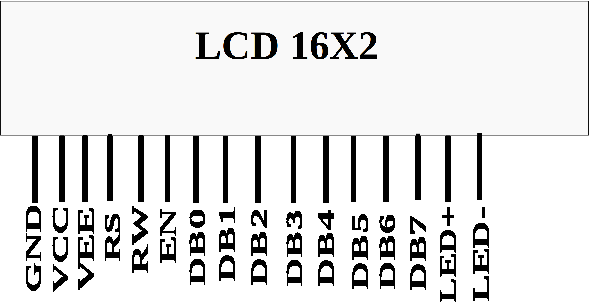
\includegraphics[scale=0.4]{figs/lcd.png}   \\
\centering
\caption{LCD 16X2}
\end{figure}

\vspace{10 cm}
\section*{\large Software}
Make the connections and connect the Vaman board to the PC via USB. In the location of choice, type the below commands
\begin{enumerate}
\item[]\url{svn co https://github.com/kkousar/KOUSAR_FWC/tree/main/arm/LCD}
\end{enumerate}
\begin{enumerate}
\item $cd LCD/GCC_Project$
\item $make$
\item $cd ../../$

\item $bash scp\_send.sh GCC_project$
\end{enumerate}




\end{document}


